\section{Results}
\label{sec:results}

% ==================================================================
% STATUS (remove before submission): all ten subsections written in
% full, every number sourced from PAPER_HANDOFF.md at time of writing
% (2026-09-03) rather than from conversational memory. Not yet done:
% (1) a human read-through end to end for flow/tone, (2) an Overleaf
% compile check (no local LaTeX engine was available to verify this),
% (3) resolving the \cite{} placeholder keys in notation.tex against
% Mendeley, (4) the abstract in main.tex, still a placeholder.
% ==================================================================

Table~\ref{tab:headline} summarises the quantitative claims this section supports, together
with the results that do \emph{not} reach significance. Each is derived in the subsection
indicated.

\begin{table}[t]
\centering
\small
\begin{tabular}{@{}llccl@{}}
\toprule
Quantity & Window & Model & Benchmark & Paired difference \\
\midrule
ACC & leads 1--18 & 0.619 & 0.565 & $+0.054$ [$+0.003$, $+0.104$] \textbf{sig.} \\
ACC & leads 8--19 & 0.480 & 0.421 & $+0.059$ [$-0.009$, $+0.127$] n.s. \\
El Ni\~no AUC & leads 12--17 & 0.825 & 0.722 & $+0.104$ [$+0.027$, $+0.196$] \textbf{sig.} \\
La Ni\~na AUC & leads 12--17 & 0.685 & 0.675 & $+0.010$ [$-0.053$, $+0.085$] n.s. \\
DJF ACC & lead 12 & 0.572 & 0.477 & $+0.095$ [$+0.007$, $+0.178$] \textbf{sig.} \\
JJA ACC & lead 18 & 0.218 & 0.283 & $-0.065$ [$-0.198$, $+0.048$] n.s. \\
ACC$=0.5$ crossing & --- & 12.4\,mo & 9.8\,mo & $+2.61$ [$-0.33$, $+9.93$] n.s. \\
Amplitude slope & lead 6 & 0.516 & 0.446 & (see Sec.~\ref{sec:amplitude-tradeoff}) \\
\bottomrule
\end{tabular}
\caption{Headline results. All intervals are 95\%, from a paired year-block bootstrap
(Sec.~\ref{sec:validation}). Results that do not reach significance are reported alongside
those that do; in particular the ACC$=0.5$ crossing, the most quotable single number, is not a
significant improvement and is not used as a claim in this paper.}
\label{tab:headline}
\end{table}

\subsection{Autoencoder fidelity}
\label{sec:ae-fidelity}

A 32-dimensional code compressing a $13\times161\times681$ field discards most of its
sub-degree structure; the relevant question is not whether information is lost, but whether
the quantities the model is scored on survive the round trip. Figure~\ref{fig:ae-fidelity}
answers this directly.

\begin{figure}[t]
  \centering
  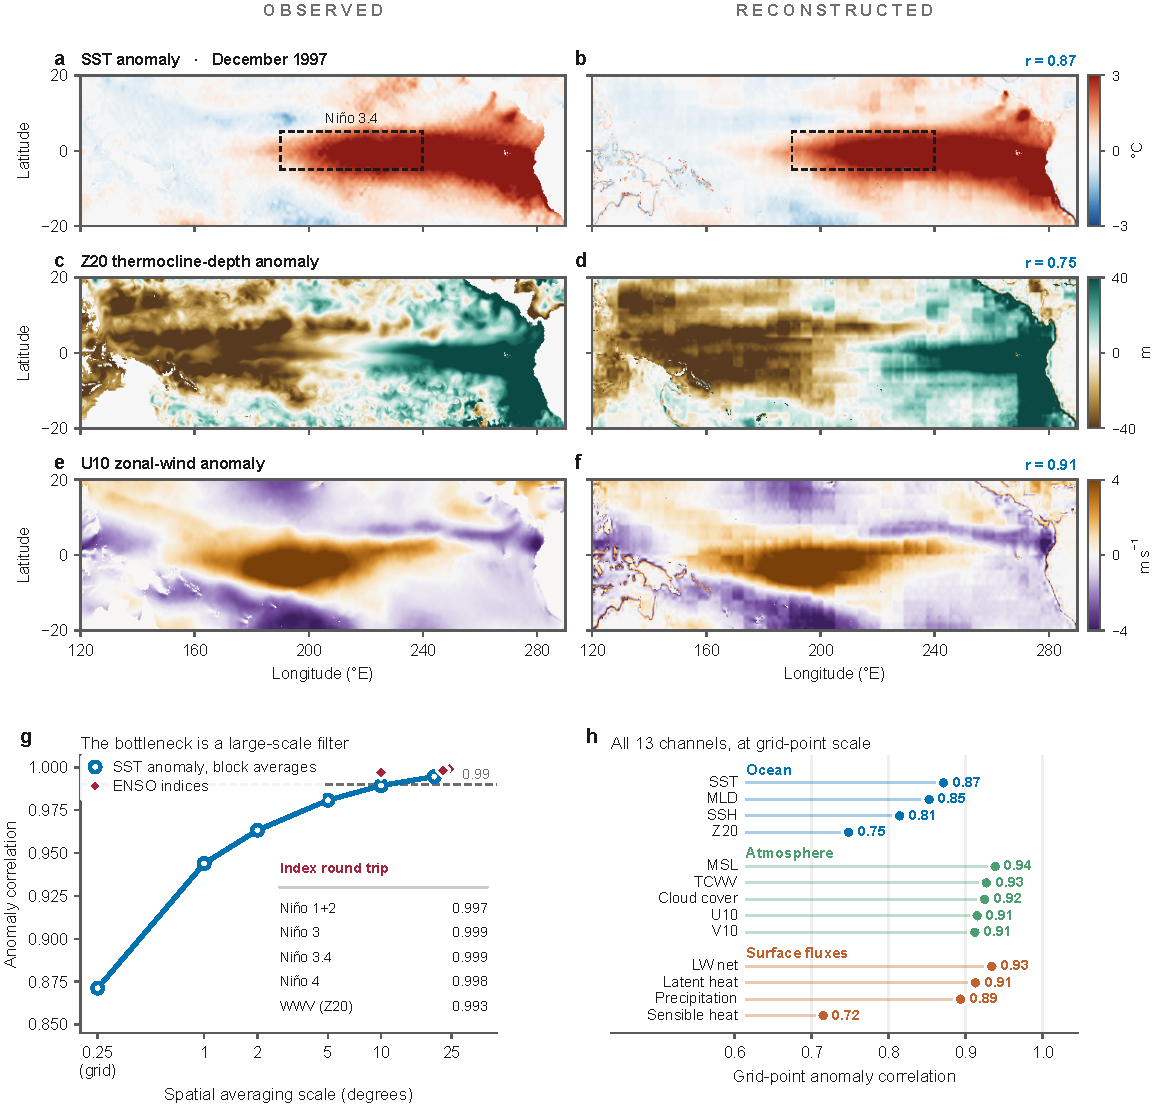
\includegraphics[width=\textwidth]{figures/fig02_ae_reconstruction.pdf}
  \caption{Autoencoder reconstruction fidelity. \textbf{(a)--(f)} Observed and reconstructed
  anomaly at the December 1997 El Ni\~no peak for SST, Z20 (thermocline depth), and U10 (zonal
  wind). \textbf{(g)} SST anomaly correlation as a function of spatial averaging scale, with
  the standard Ni\~no indices placed at the effective scale of their own averaging box.
  \textbf{(h)} Grid-point anomaly correlation for all 13 channels, grouped by ocean,
  atmosphere, and surface flux.}
  \label{fig:ae-fidelity}
\end{figure}

Reconstruction fidelity is scale-dependent: SST anomaly correlation is 0.871 at the native
$0.25\deg$ grid, rising to 0.944 at $1\deg$, 0.981 at $5\deg$, and 0.995 at $20\deg$ averaging.
The bottleneck discards sub-degree structure and retains the large scale. Both quantities the
model forecasts survive this round trip well above the grid-point level: Ni\~no 3.4 reaches
ACC $0.999$, RMSE $0.047\deg$C, amplitude ratio $0.990$; WWV reaches ACC $0.993$, RMSE
$0.78\,\mathrm{m}$, amplitude ratio $0.969$. The autoencoder is therefore not the limiting
factor for the skill reported in the remainder of this section.

Across all 13 channels, grid-point anomaly correlation ranges from 0.715 (sensible heat flux,
small-scale and noisy) and 0.748 (Z20, which has sharp thermocline gradients) up to 0.938
(mean sea-level pressure); amplitude ratios are within $0.94$--$1.12$ for every channel, so the
autoencoder is not systematically damping or inflating variance. Two artefacts are visible in
the reconstructed fields at fine scale -- thin dipole fringes along coastlines, from the
decoder's limited resolution of the land mask, and faint rectangular blocking in the far
western Pacific, from the $4\times4$ patch structure of the decoder -- neither of which
intersects the Ni\~no boxes.

\subsection{What the latent coordinates are}
\label{sec:latent-coords}

\begin{figure}[t]
  \centering
  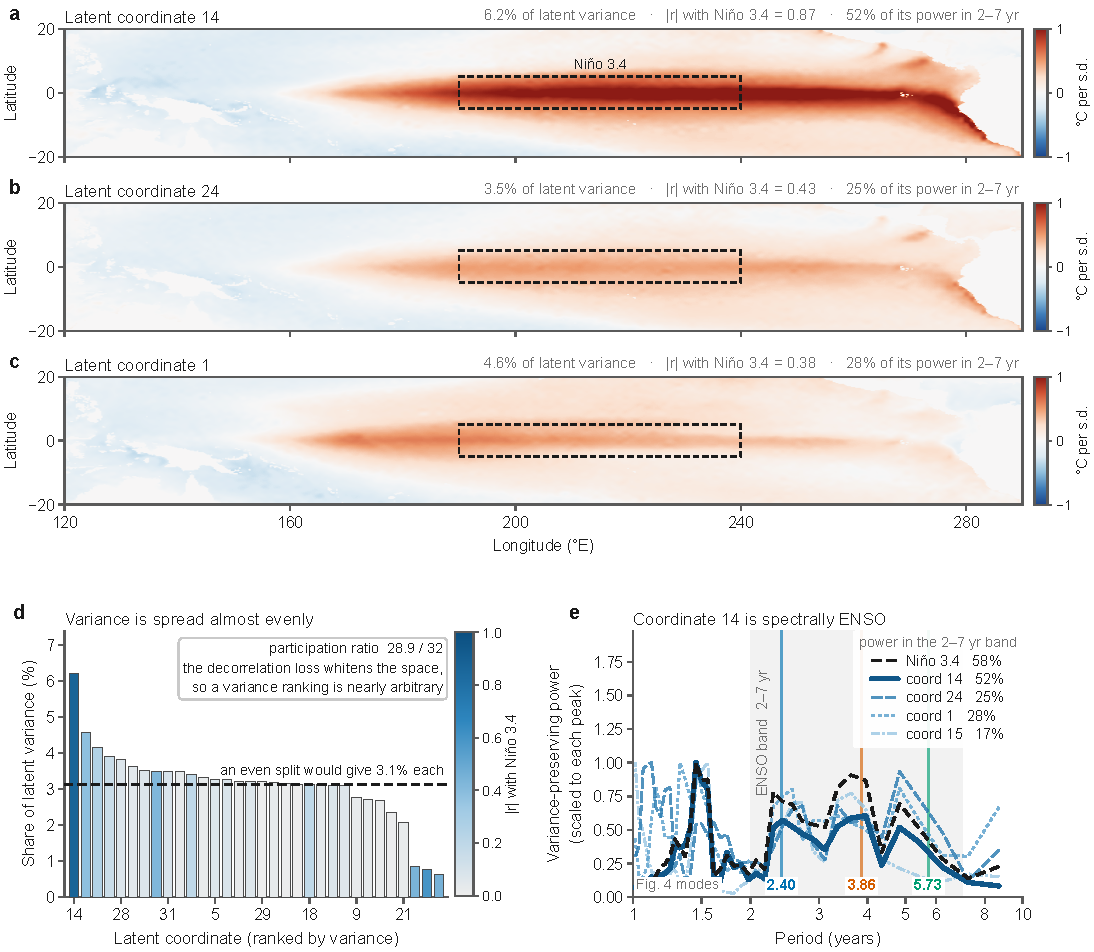
\includegraphics[width=\textwidth]{figures/fig03_latent_space.pdf}
  \caption{The latent coordinates. \textbf{(a)--(c)} SST-anomaly regression footprints (degC
  per standard deviation of the coordinate) for the three coordinates with above-average
  variance share and the strongest association with Ni\~no 3.4. \textbf{(d)} Variance share of
  all 32 coordinates, shaded by $|r|$ with Ni\~no 3.4. \textbf{(e)} Multitaper spectra of the
  leading coordinates against Ni\~no 3.4, on the same period axis and estimator as
  Fig.~\ref{fig:modal-spectrum}.}
  \label{fig:latent-coords}
\end{figure}

The latent space is close to isotropic: its participation ratio is 28.9 of 32, and the
coordinate with the largest variance share holds only 6.22\%, against 3.13\% for a perfectly
even split -- consistent with the decorrelation and $\ell_2$ penalties applied during training.
A consequence is that ranking coordinates by variance alone selects near-arbitrary directions;
Fig.~\ref{fig:latent-coords} instead selects coordinates with above-average variance share
\emph{and} the strongest association with Ni\~no 3.4.

By that criterion, ENSO is concentrated in essentially one coordinate. Coordinate 14 has the
largest variance share (6.22\%), the strongest correlation with Ni\~no 3.4 ($r=-0.874$), and
the largest fraction of its spectral power in the 2--7 year ENSO band (0.523, close to Ni\~no
3.4's own 0.578); its spatial footprint is the canonical cold-tongue/equatorial-warming
pattern. Only 2 of the 32 coordinates exceed $|r|=0.5$ with Ni\~no 3.4. Two further
coordinates, 1 and 24, carry secondary, weaker ENSO-associated patterns ($r=+0.383$ and
$-0.425$ respectively, 25--28\% of their power in the ENSO band). A spectral peak near 1.45
years, present in every leading coordinate and in Ni\~no 3.4 itself, is the ENSO$\times$annual
combination tone discussed in Sec.~\ref{sec:modal-spectrum}, not a latent-space artefact.

This concentration describes the \emph{output} the latent state produces, not the state needed
to produce it: Sec.~\ref{sec:ablations} shows that restricting the forecast operator to a
subspace built from ENSO-correlated coordinates costs forecast skill, so the remaining
coordinates -- individually weakly correlated with Ni\~no 3.4 -- carry predictive information
about how coordinate 14 will evolve.

\subsection{The modal spectrum}
\label{sec:modal-spectrum}

\begin{figure}[t]
  \centering
  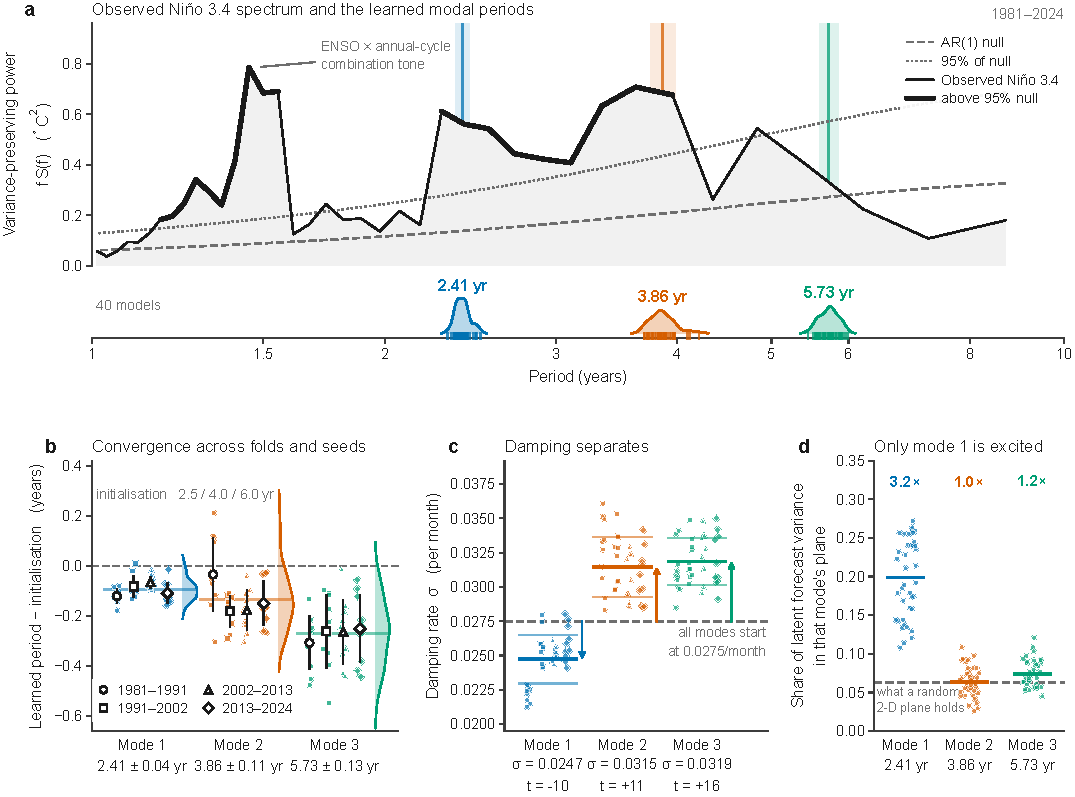
\includegraphics[width=\textwidth]{figures/fig04_modal_spectrum.pdf}
  \caption{The modal spectrum across all 40 trained models. \textbf{(a)} Multitaper spectrum of
  the observed Ni\~no 3.4 anomaly against an AR(1) red-noise null, with the operator's learned
  periods overlaid. \textbf{(b)} Learned period of each oscillator across all 40 models,
  against its initialised value. \textbf{(c)} Learned damping rate; all three oscillators begin
  training at an identical value. \textbf{(d)} Fraction of latent forecast variance projecting
  onto each oscillator's 2-D plane, against the value expected for an isotropic state.}
  \label{fig:modal-spectrum}
\end{figure}

All 40 trained models (4 folds $\times$ 10 seeds) converge on the same three periods:
$2.405\pm0.041$, $3.864\pm0.115$, and $5.729\pm0.127$ years, with damping rates
$0.0247\pm0.0018$, $0.0315\pm0.0022$, and $0.0319\pm0.0017$ per month respectively. Three
properties of this result require care in interpretation.

First, the periods are initialised in-band, at 2.5, 4.0, and 6.0 years, identically in every
run, so they do not emerge without spectral supervision; what is observed is a consistent,
statistically significant displacement from that initialisation across four disjoint training
epochs ($t(39)=-14.5$, $-7.5$, $-13.4$ for modes 1--3), with no learned period sitting at the
$[1,10]$-year bound the parameterisation allows. Second, stability is imposed rather than
learned: the damping parameterisation guarantees $\sigma_k>0$, so no mode can grow, and this
must not be read as a learned property. What \emph{is} learned is the magnitude and ordering
of the damping: all three oscillators begin training at an identical damping of
$0.0275\,\mathrm{month}^{-1}$ and separate over training ($t(39)=-9.9$, $+11.4$, $+15.9$), with
the 2.41-year mode becoming the least damped. Because the three dampings start identical while
the periods start separated, this separation is the strongest emergent result in the figure.

Third, and most consequential for how this spectrum should be read: only the leading mode is
dynamically active. Projecting the latent forecast onto each oscillator's 2-D plane (an
isotropic 32-dimensional state would place a fraction $2/32=0.062$ in any such plane), the
2.41-year mode carries $0.199\pm0.051$ of forecast variance ($3.2\times$ the isotropic
baseline); the 3.86- and 5.73-year modes carry $0.064\pm0.019$ and $0.074\pm0.018$
($1.0\times$ and $1.2\times$ baseline, i.e.\ not excited above what an isotropic state would
show). The 5.73-year mode fails three further, independent tests: it sits below the 95\%
AR(1) significance level of the observed spectrum (0.399 against 0.554); its period shows no
sensitivity to which decade it is trained on ($F(3,36)=0.36$, against $F=4.80$ and $4.64$,
$p<0.01$, for modes 1 and 2); and it is not excited, as above. It should not be presented as an
established third ENSO band.

The observed Ni\~no 3.4 spectrum (deseasonalised, linearly detrended, $N=522$ months;
multitaper, $NW=2$, $K=3$; AR(1) null matched in variance and lag-1 autocorrelation; 95\% level
from a $\chi^2$ distribution with $2K=6$ degrees of freedom) has one contiguous band exceeding
the 95\% level, at 2.29--3.95 years. The 2.41- and 3.86-year modes lie inside this band; the
5.73-year mode does not. A spectral peak near 1.4--1.5 years, present in the observed spectrum
and in every leading latent coordinate (Sec.~\ref{sec:latent-coords}), is consistent with the
ENSO$\times$annual-cycle combination tone predicted at $1/(1/12\pm1/T)$ for $T=3.9$ years
(giving 1.34 years), and is robust to linear or quadratic detrending.

The defensible summary is one dominant quasi-biennial oscillator at $2.41\pm0.04$ years, plus
damped memory, rather than three independently established ENSO bands. Whether this
three-oscillator structure itself is necessary -- as opposed to an artefact of a hardcoded
choice -- is tested directly in Sec.~\ref{sec:ablations}.

\subsection{Deterministic skill versus lead}
\label{sec:skill}

Figure~\ref{fig:skill} shows anomaly correlation, the paired model$-$benchmark difference, and
normalised RMSE as a function of lead, for the model, the observable-predictor benchmark, and
persistence.

\begin{figure}[t]
  \centering
  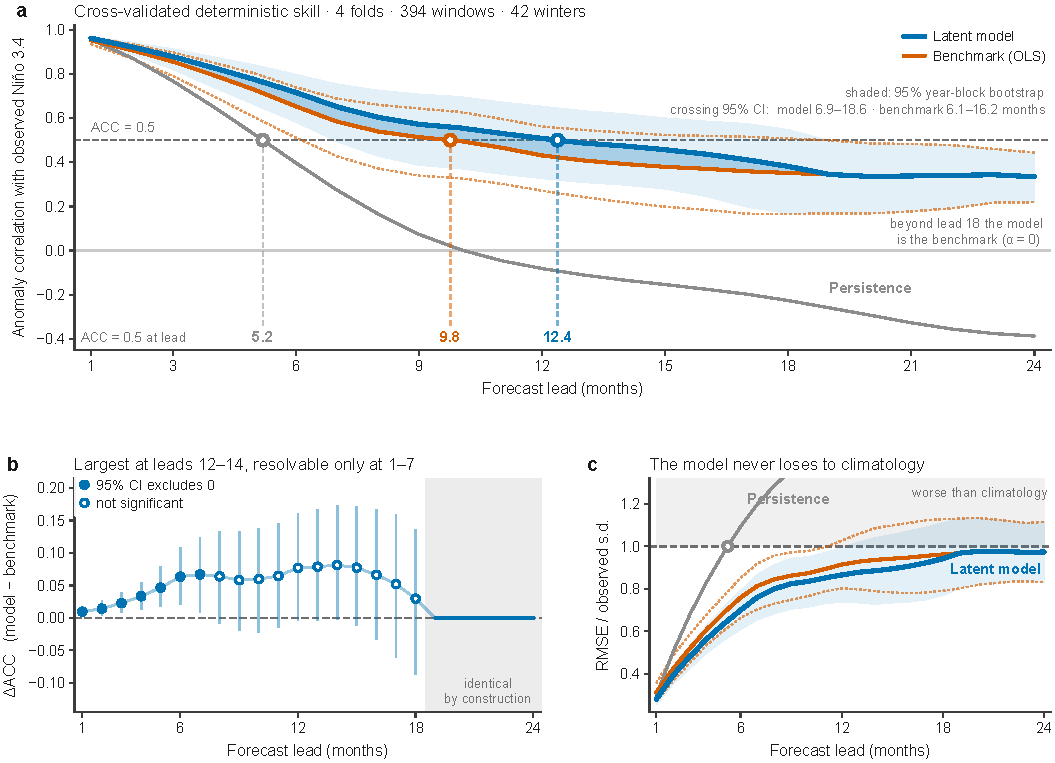
\includegraphics[width=\textwidth]{figures/fig05_skill_vs_lead.pdf}
  \caption{Deterministic skill against lead time. \textbf{(a)} Anomaly correlation of the
  model, the benchmark, and persistence, with 95\% paired year-block bootstrap bands and the
  ACC$=0.5$ crossings shown with their own confidence intervals. \textbf{(b)} The paired
  model$-$benchmark difference; leads 19--24 are identically zero by construction
  ($\alpha(l)=0$ there) and are shaded. \textbf{(c)} RMSE normalised by the per-lead observed
  standard deviation, so that 1.0 corresponds to a climatological forecast.}
  \label{fig:skill}
\end{figure}

Over leads 1--18, mean ACC is 0.619 for the model against 0.565 for the benchmark, a paired
difference of $+0.054$ [$+0.003$, $+0.104$], significant at 95\%. Per-lead, the model
significantly exceeds the benchmark at leads 1--7 (lead 8 is borderline: $+0.064$
[$-0.009$, $+0.132$]); it significantly exceeds persistence at leads 2--24. The gain is
front-loaded in significance but largest in absolute terms at intermediate lead, reaching
$+0.077$ to $+0.081$ at leads 12--14, where it is not significant because the bootstrap
interval widens with lead. By construction, $\alpha(l)=0$ for $l>18$, so the model and
benchmark are identical over leads 19--24 and their paired difference is exactly zero at every
one of those leads -- a consequence of the blend weight, not a null result.

The ACC$=0.5$ crossing is 12.38 months [6.93, 18.60] for the model against 9.76
[6.14, 16.18] for the benchmark, a gain of $+2.61$ months [$-0.33$, $+9.93$] that does
\emph{not} exclude zero. This crossing is a threshold statistic -- it reads off where a noisy
curve intersects a fixed level, so a small fluctuation in ACC moves it disproportionately --
and it is reported here as descriptive rather than as a claim of significance; the leads 1--18
mean difference and the per-lead significance above are the results this paper's claims rest
on.

Normalised RMSE (Fig.~\ref{fig:skill}c) never reaches 1.0 for either the model or the
benchmark within the 24-month window (peaking at 0.976 near lead 20), so neither forecast is
worse than climatology at any lead considered, though the margin is negligible beyond
$\sim$lead 18. Persistence, by contrast, crosses 1.0 at lead 5.2 and continues to rise. By
lead~12, both the model and the benchmark have decayed to approximately the observed spread in
RMSE terms while ACC remains near 0.5: the forecast retains phase information for longer than
it retains amplitude, a point developed quantitatively in Sec.~\ref{sec:amplitude-tradeoff}.

\subsection{Event discrimination}
\label{sec:event-auc}

Event thresholds in this section are $\pm1.0\deg$C, not the conventional $\pm0.5$ ONI
threshold; this must be stated explicitly, as no number below reproduces under the
conventional definition. Over 1981--2024 this threshold yields 11 distinct El Ni\~no episodes
(69 months) and 14 La Ni\~na episodes (64 months); the effective sample size for significance
is therefore episodes, not the 46 and 58 verification windows per lead that meet the threshold,
which are not independent of one another.

\begin{figure}[t]
  \centering
  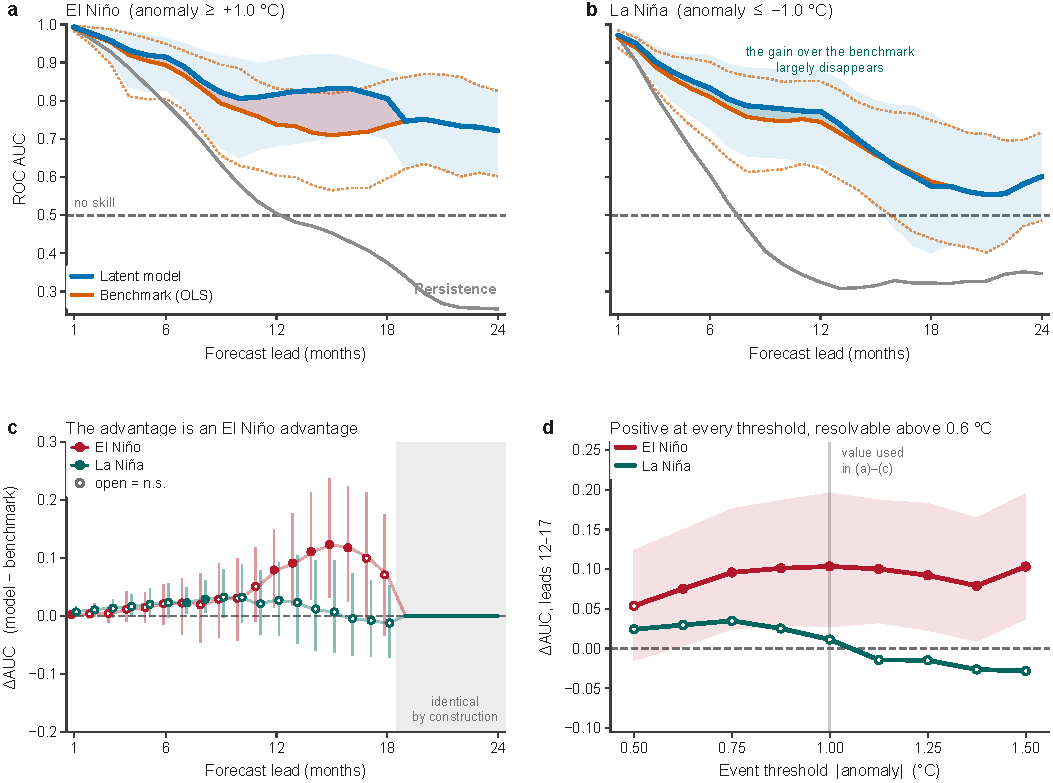
\includegraphics[width=\textwidth]{figures/fig06_event_auc.pdf}
  \caption{Event discrimination by ROC area under the curve (Mann--Whitney statistic;
  for La Ni\~na the score is negated so that higher always indicates a more likely event).
  \textbf{(a)} El Ni\~no AUC against lead. \textbf{(b)} La Ni\~na AUC. \textbf{(c)} Paired
  model$-$benchmark differences with 95\% bootstrap intervals. \textbf{(d)} Sensitivity of the
  leads 12--17 difference to the event threshold, 0.5 to $1.5\deg$C.}
  \label{fig:event-auc}
\end{figure}

Over leads 12--17, El Ni\~no AUC is 0.825 for the model against 0.722 for the benchmark, a
paired difference of $+0.104$ [$+0.027$, $+0.196$], significant at 95\%; over leads 8--18 the
difference is $+0.075$ [$+0.016$, $+0.142$], also significant. Per lead, the El Ni\~no
difference is significant at lead 1 and at leads 12--16, but not at leads 2--11 or 17--18. La
Ni\~na AUC is lower in absolute terms (0.685 against 0.825 for El Ni\~no at leads 12--17), and
the gain over the benchmark is not distinguishable from zero at any lead beyond 7--8 (leads
12--17: $+0.010$ [$-0.053$, $+0.085$]; leads 8--18: $+0.015$ [$-0.031$, $+0.069$]). Both
phases significantly exceed persistence at long lead: El Ni\~no at leads 6--24, La Ni\~na at
leads 2--24.

The model's advantage over the benchmark is therefore an El Ni\~no advantage. This is
consistent with the sign-symmetry of a linear operator (Sec.~\ref{sec:architecture}), which
has no mechanism to represent an asymmetric response to warm and cold anomalies, appearing
here as a measured quantity rather than an architectural assertion. Panel (d) shows this is not
an artefact of the $\pm1.0\deg$C threshold: the El Ni\~no gain is positive at every threshold
tested, 0.5 to $1.5\deg$C, and significant from $0.625\deg$C upward, but at the conventional
$0.5\deg$C threshold it is $+0.054$ [$-0.015$, $+0.124$], not significant -- the model's
event-discrimination gain is specific to substantial events, and the record cannot resolve it
at the weak-event threshold. Above approximately $1.05\deg$C the La Ni\~na difference turns
negative ($-0.014$ to $-0.028$): the operator's residual mildly reduces skill for the
strongest cold events.

\subsection{Seasonality of skill}
\label{sec:seasonality}

\begin{figure}[t]
  \centering
  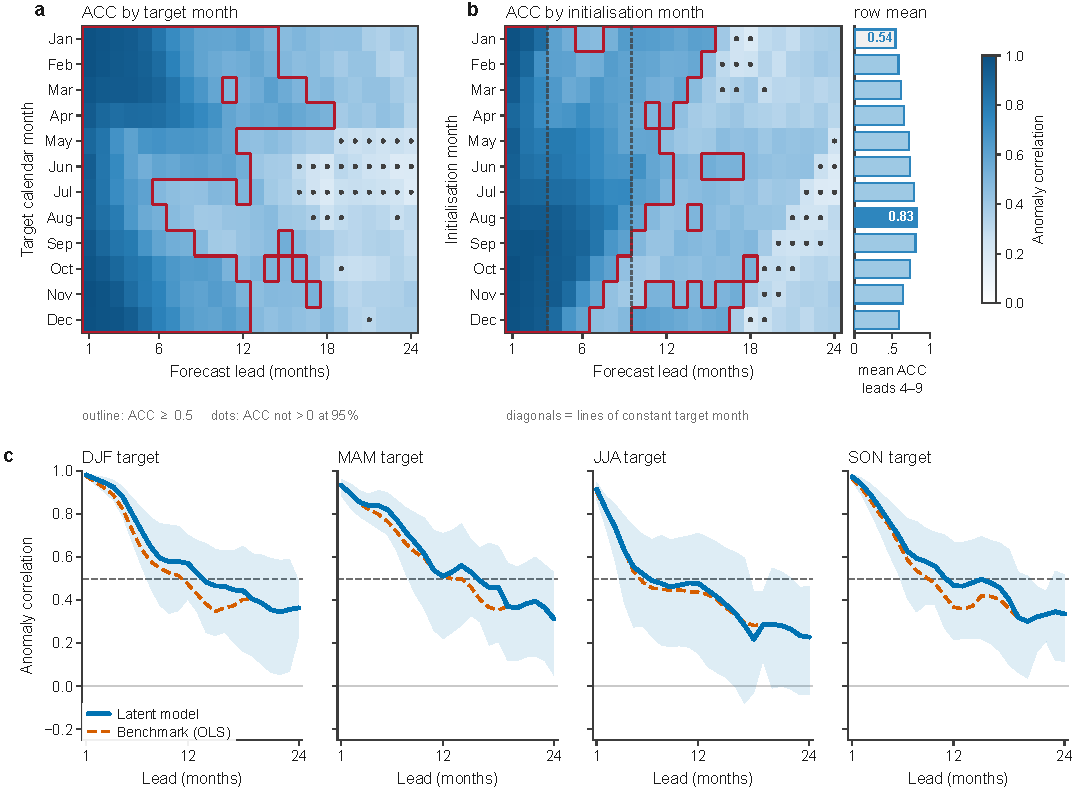
\includegraphics[width=\textwidth]{figures/fig07_seasonality.pdf}
  \caption{Seasonality of skill. \textbf{(a)} ACC by target calendar month and lead; stippling
  marks the 30 of 288 cells where ACC is \emph{not} significantly above zero. \textbf{(b)} The
  same skill by initialisation month; diagonals are lines of constant target month.
  \textbf{(c)} The four target seasons, model against benchmark, with 95\% confidence
  intervals.}
  \label{fig:seasonality}
\end{figure}

ACC is significantly above zero in 258 of the 288 target-month$\times$lead cells; the
stippling in Fig.~\ref{fig:seasonality}a marks the 30 cells that are not, rather than the
(near-total) majority that are. Averaged over leads 4--9, target-month skill is strongest for
March (ACC $0.829$) and weakest for August ($0.509$); the region where ACC is not significantly
positive is concentrated in May--August targets beyond approximately lead 16, consistent with
ENSO's tendency to peak in boreal winter.

Skill viewed by initialisation month (Fig.~\ref{fig:seasonality}b) follows the same pattern,
because it is the same information under a different projection: since target month equals
initialisation month plus lead for every window, panel (b) is an exact shear of panel (a) --
verified numerically, with the two grids identical once one is sheared onto the other's
coordinates -- and contains no information panel (a) does not. Initialising in August
verifies well because leads 4--9 from an August initialisation land on December through May
targets, the predictable winter/spring window; initialising in January verifies poorly because
the same lead window lands on May through October, the summer dead zone. This is not evidence
of an information loss specific to the boreal-spring transition -- target month, initialisation
month, and lead are linearly dependent in this grid, so such a claim cannot be tested from it --
and panel (b) should be read as an operationally useful view of the target-month result in
panel (a), not as independent evidence for a spring predictability barrier.

Per-cell model-versus-benchmark significance is not shown on the heat maps: only 28 of 288
cells pass at $p<0.05$, close to the $\sim$14 expected by chance under repeated pointwise
testing, and would be misleading if stippled. The comparison is instead made at the seasonal
level in Fig.~\ref{fig:seasonality}c. The model's per-lead gain over the benchmark is
significant at long range only for DJF targets ($+0.095$ [$+0.007$, $+0.178$] at lead 12); MAM
shows no gain at the same lead ($-0.004$); JJA is slightly negative at lead 18 ($-0.065$, not
significant). This is the same lead window in which the El Ni\~no AUC gain peaks
(Sec.~\ref{sec:event-auc}, leads 12--17): the two results describe one effect, not two -- the
operator's residual adds skill for the mature winter phase of warm events, and adds
essentially nothing for the summer transition or for cold events.

By target season, the model's ACC confidence interval remains above 0.5 through lead 7 for
DJF, lead 8 for MAM, lead 3 for JJA, and lead 6 for SON, and remains above zero through lead 24
for DJF, MAM, and SON but only through lead 21 for JJA -- summer targets at long lead are where
the model has no demonstrable skill (ACC $0.218$ [$-0.029$, $0.438$] at lead 18), a limitation
that sits alongside the La Ni\~na asymmetry of Sec.~\ref{sec:event-auc}.

\subsection{Event case studies and the amplitude shortfall}
\label{sec:case-studies}

\begin{figure}[t]
  \centering
  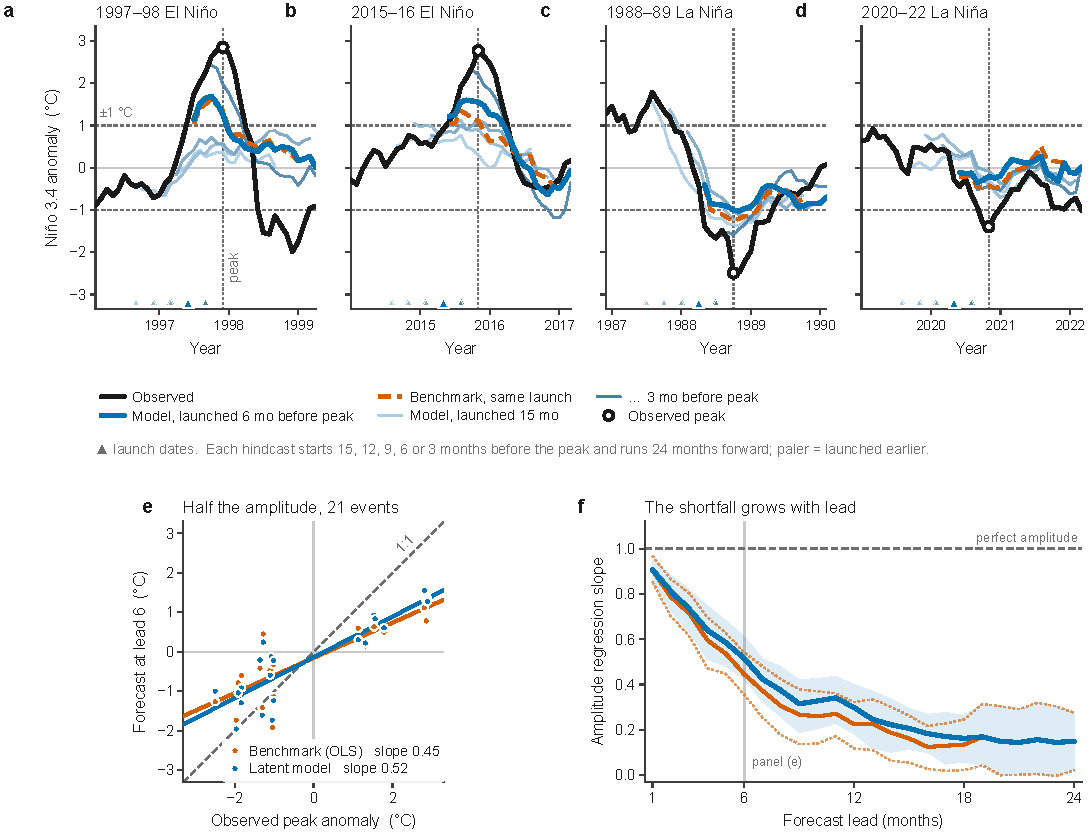
\includegraphics[width=\textwidth]{figures/fig08_case_studies.pdf}
  \caption{Event case studies and the amplitude shortfall. \textbf{(a)--(d)} Four events, each
  with the observed Ni\~no 3.4 anomaly and model hindcasts launched every three months through
  the 15 months before the peak (pale: earliest launch; dark: closest to the peak); the
  benchmark is drawn for the launch nearest six months before the peak.
  \textbf{(e)} Forecast peak against observed peak at lead 6, with the regression slope.
  \textbf{(f)} That slope as a function of lead.}
  \label{fig:case-studies}
\end{figure}

Coverage is set by the 24-month fold buffer (Sec.~\ref{sec:validation}): of 25 events with
$|\mathrm{anomaly}|\ge1.0\deg$C over 1981--2024, the 1992 and 2002 El Ni\~no events have no
hindcast coverage at all, and 2023--24 has only seven initialisations. The four events shown
were chosen for full coverage and for the range of behaviour they illustrate: the 1997--98 and
2015--16 El Ni\~nos, and the 1988--89 and 2020--22 La Ni\~nas.

Regressing forecast peak on observed peak across every event with sufficient coverage gives a
slope of $0.516$ [$0.426$, $0.612$] at lead 6 (21 events; the benchmark reaches $0.446$
[$0.356$, $0.542$]), falling systematically with lead: $0.734$ at lead 3, $0.516$ at lead 6,
$0.315$ at lead 9, $0.298$ at lead 12, $0.163$ at lead 18. Even at lead 1 the slope is $0.91$.
The three strongest observed El Ni\~nos, all near $+2.8\deg$C, illustrate the same shortfall
directly: 1983-01 (observed $+2.85$, model $+1.30$), 1997-12 (observed $+2.88$, model $+1.27$),
2015-11 (observed $+2.80$, model $+1.55$). This amplitude shortfall is quantified and explained
mechanistically in Sec.~\ref{sec:amplitude-tradeoff}: it is not a consequence of the operator
being unable to represent large anomalies, but of the published blend weight discarding
amplitude that the raw hybrid forecast already carries.

The four case studies illustrate this range of behaviour. For 1997--98, timing is captured from
approximately nine months before the peak, and the six-month-ahead launch reaches
$+1.7\deg$C against an observed $+2.9\deg$C; the model then largely misses the transition into
the 1998--99 La Ni\~na. The 2015--16 event is the best-captured extreme, reaching $+1.55$ at
lead 6 with the subsequent decay through 2016 tracked. The 1988--89 La Ni\~na, the strongest
cold event in the record, reaches approximately $-1.3\deg$C against an observed $-2.5\deg$C at
lead 6. The 2020--22 multi-year La Ni\~na is the weakest case: the lead-6 forecast is $-0.21$
against an observed $-1.40\deg$C, and the model stays close to zero while the event persists --
the same multi-year, La Ni\~na-specific weakness quantified in Sec.~\ref{sec:event-auc}, shown
here rather than omitted.

\subsection{The forecast in physical space}
\label{sec:physical-space}

Every result so far concerns the Ni\~no 3.4 and WWV indices. Because the latent forecast
decodes to full physical fields, skill can also be assessed spatially, by decoding the stored
latent \emph{forecasts} (as opposed to the reconstructions of Sec.~\ref{sec:ae-fidelity})
through the frozen decoder.

\begin{figure}[t]
  \centering
  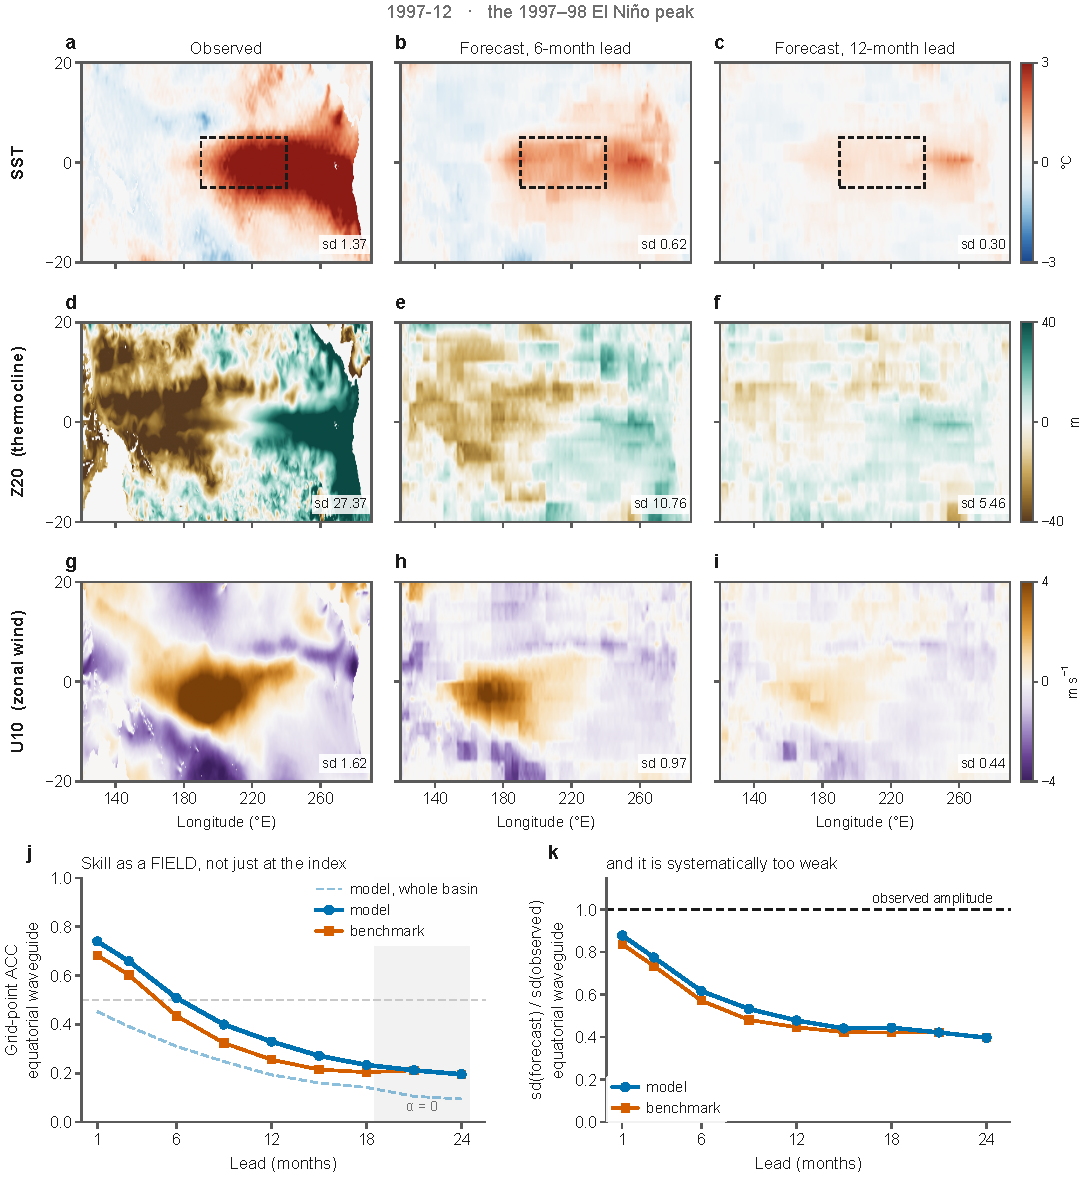
\includegraphics[width=\textwidth]{figures/fig09_physical_forecast.pdf}
  \caption{The forecast in physical space. \textbf{(a)--(i)} Observed anomaly at the December
  1997 El Ni\~no peak alongside the model forecast for that month launched 6 and 12 months
  earlier, for SST, Z20, and U10. \textbf{(j)} Grid-point anomaly correlation, area-weighted
  over the equatorial waveguide ($5\deg$S--$5\deg$N, $160\deg$E--$80\deg$W), against lead, for
  the model and the benchmark. \textbf{(k)} The ratio of forecast to observed spatial standard
  deviation against lead.}
  \label{fig:physical-space}
\end{figure}

Averaged over the equatorial waveguide, where the ENSO signal is concentrated, grid-point
anomaly correlation is 0.740 at lead 1, falling to 0.508 at lead 6, 0.330 at lead 12, and
0.196 at lead 24, with the model exceeding the benchmark by $+0.05$ to $+0.08$ at every lead
where $\alpha>0$. A whole-basin average, by contrast, is approximately 0.3 lower at short lead
(0.452 against 0.740 at lead 1) because it dilutes the signal with ocean that carries no ENSO
information, and is not the quantity any claim in this paper rests on.

Z20 (thermocline depth) is forecast as well as SST at every lead shown (both reach ACC $0.58$
at lead 6), even though the model is trained and scored on Ni\~no 3.4 and WWV rather than on
the spatial field directly: the recharge-oscillator memory is being predicted, not only the
surface signature. This is independent, physical-space support for
Sec.~\ref{sec:ablations}'s finding that the full latent state, not an ENSO-correlated subspace,
is required for forecasting. The model's advantage over the benchmark is, if anything, larger
in field space than at the index -- approximately $+0.075$ and roughly flat over leads 6--15,
against $+0.063$ at lead 6 for Ni\~no 3.4 alone -- consistent with the benchmark's four scalar
predictors reconstructing the index tolerably but the spatial pattern poorly.

The amplitude ratio (Fig.~\ref{fig:physical-space}k) falls from $0.879$ at lead 1 to $0.617$ at
lead 6 and $0.479$ at lead 12, flattening near $0.40$ by lead 24 even as ACC continues to fall
to $0.196$: at long lead the forecast retains amplitude for longer than it retains phase, the
converse of the pattern noted for RMSE in Sec.~\ref{sec:skill}. The model is consistently less
damped than the benchmark at every lead where $\alpha>0$ ($0.617$ against $0.572$ at lead 6),
though not enough to close the gap. Part of the shortfall at lead 1 ($0.879$, not $1.0$) is
attributable to the autoencoder rather than the dynamics, since the grid-point SST
reconstruction ceiling itself is $0.871$ (Sec.~\ref{sec:ae-fidelity}).

\subsection{Ablations}
\label{sec:ablations}

Three architectural choices are tested directly against alternatives, each defending a design
decision with a measurement rather than an assumption.

\paragraph{Latent dimension.} Restricting the operator to an 8-dimensional subspace built from
the coordinates most correlated with Ni\~no 3.4 (fold 3, 3 seeds; 16{,}898 parameters against
79{,}682 for the full operator) costs $-0.068$ mean ACC (leads 1--18) and $-0.137$ at lead 12,
well outside the $0.03$--$0.04$ seed-to-seed spread measured for this configuration. This
appears to contradict Sec.~\ref{sec:latent-coords}, where ENSO's \emph{output} is shown to be
concentrated in one coordinate, but the two results answer different questions: the other
$\sim$24 coordinates are poor linear projections onto Ni\~no 3.4 but carry information the
operator uses to predict how the ENSO-correlated coordinate will evolve, consistent with
recharge-oscillator theory, in which thermocline structure rather than SST itself is the
memory that sets future SST. The defensible statement is that ENSO's forecast \emph{output} is
one-dimensional, but the \emph{state} required to forecast it is not.

\paragraph{Oscillator count.} The operator's three oscillators (Sec.~\ref{sec:modal-spectrum})
were fixed at model-development time and never varied against alternatives. A single-fold
development experiment (fold 3, 6 paired seeds) found that adding a fourth oscillator
initialised at 1.4 years -- a period corresponding to a genuine, well-constrained spectral
feature (Sec.~\ref{sec:modal-spectrum}) -- improved mean ACC by $+0.0124$ (SE $0.0021$,
$t=5.93$, 6 of 6 seeds better). Retraining both the three- and four-oscillator configurations
across all four folds and ten seeds, paired, does not confirm this: the pooled difference over
40 paired runs is $+0.0030\pm0.0145$ ($t=1.31$), with only 20 of 40 seed-fold pairs favouring
the four-oscillator configuration and the sign of the effect reversing between folds. The
effect survives only on the fold that selected the configuration -- a textbook case of
selection bias, here measured rather than merely warned against, and the reason this paper
reports skill from folds distinct from the fold used for model development
(Sec.~\ref{sec:validation}). The three-oscillator configuration is retained unchanged. The
1.4-year period itself is stable and well-determined across all 40 four-oscillator runs
(1.37--1.52 years), so the spectral feature is real and representable; it simply does not
improve forecast skill.

\paragraph{An explicit amplitude nonlinearity.} Because the amplitude shortfall of
Sec.~\ref{sec:case-studies} suggests a damped linear operator may be unable to grow an
anomaly, a bounded, learnable nonlinear term was added inside the monthly recursion, in each
oscillator's own two-dimensional plane, permitting both self-amplification (capped at 5\% per
month, corresponding to a $1.5$--$2.2\times$ range over 24 months) and a quadratic term
capable of breaking the sign symmetry noted in Sec.~\ref{sec:event-auc}. Both terms are
zero-initialised. Trained and evaluated with the same paired, six-seed protocol, the
nonlinearity changes mean ACC by $-0.0000\pm0.0008$ and the lead-6 amplitude slope from
$0.470$ to $0.468$ -- no measurable effect. Given the capacity to amplify, the learned
self-amplification coefficients are negative in five of six oscillator instances, corresponding
to \emph{additional} damping (24-month amplitude factors of $0.98\times$ down to
$0.71\times$). The amplitude shortfall is therefore not a structural property of a damped
linear operator, which was given, and declined, the means to grow anomalies; its actual
mechanism is identified in Sec.~\ref{sec:amplitude-tradeoff}.

\subsection{The amplitude--correlation trade}
\label{sec:amplitude-tradeoff}

Section~\ref{sec:ablations} closes two candidate explanations for the amplitude shortfall of
Sec.~\ref{sec:case-studies} without improving skill: neither the number of oscillators nor an
explicit amplitude nonlinearity accounts for it. What remains is the blend itself
(Sec.~\ref{sec:blend}), and because the blend is linear in $\alpha$, its contribution to both
skill and amplitude can be characterised exactly using only the benchmark and raw hybrid
forecasts already computed for every verification window, without retraining.

\begin{figure}[t]
  \centering
  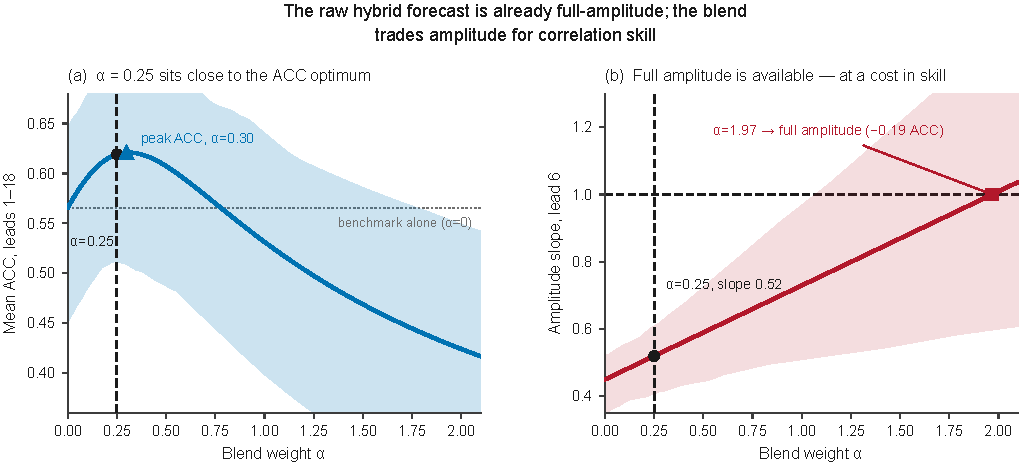
\includegraphics[width=\textwidth]{figures/fig10_alpha_tradeoff.pdf}
  \caption{The blend weight as a variance--correlation trade. \textbf{(a)} Mean ACC over leads
  1--18 as a function of $\alpha$, with 95\% bootstrap bands; $\alpha=0.25$, the weight used
  throughout this study, and the ACC-maximising $\alpha=0.30$ are marked and nearly coincide.
  \textbf{(b)} The amplitude regression slope at lead 6 as a function of $\alpha$ -- exactly
  linear, since the blended forecast is a linear combination of the benchmark and the raw
  hybrid forecast -- with the $\alpha$ that restores full amplitude (slope $=1$) marked
  together with its cost in ACC.}
  \label{fig:amplitude-tradeoff}
\end{figure}

\begin{table}[t]
\centering
\begin{tabular}{@{}lccl@{}}
\toprule
$\alpha$ & ACC, leads 1--18 & Amplitude slope, lead 6 & \\
\midrule
0.00 & 0.5654 & 0.451 & benchmark alone \\
\textbf{0.25} & \textbf{0.6191} & 0.519 & used throughout this study \\
0.30 & 0.6209 & 0.529 & ACC-maximising \\
1.00 & 0.5314 & \textbf{0.729} & raw hybrid, unblended \\
1.97 & 0.4265 & \textbf{1.000} & exact, full amplitude \\
\bottomrule
\end{tabular}
\caption{Skill and amplitude as a function of the blend weight $\alpha$.}
\label{tab:alpha-sweep}
\end{table}

At $\alpha=1$ -- the raw, unblended hybrid forecast -- amplitude slope at lead 6 is $0.729$,
exceeding the $0.519$ obtained at $\alpha=0.25$. The blend does not fail to produce amplitude;
it is constructed to discard most of it, because $\alpha=0.25$ sits close to what maximises
ACC ($\alpha=0.30$; the $+0.0018$ difference between them is within the seed-to-seed spread of
$0.0053$ established in Sec.~\ref{sec:ablations} and is not grounds to prefer a different
weight).

Because $P(\alpha)=\mathrm{benchmark}+\alpha(\mathrm{hybrid}-\mathrm{benchmark})$ is linear in
$\alpha$, the amplitude slope is exactly linear in $\alpha$ as well, and the value of $\alpha$
that restores full amplitude at lead 6 can be solved for directly:
\[
\mathrm{slope}(\alpha) = \frac{\mathrm{cov}(\mathrm{benchmark},\,\mathrm{truth})}
{\mathrm{var}(\mathrm{truth})} + \alpha\,\frac{\mathrm{cov}(\mathrm{hybrid}-
\mathrm{benchmark},\,\mathrm{truth})}{\mathrm{var}(\mathrm{truth})}
= 0.4494 + 0.2798\,\alpha,
\]
giving $\alpha \approx 1.968$ for $\mathrm{slope}=1.0$, at which mean ACC (leads 1--18) is
$0.4265$ -- a cost of $0.19$ relative to $\alpha=0.25$, larger than every skill gain reported
elsewhere in this paper.

This resolves the amplitude shortfall of Sec.~\ref{sec:case-studies} and the retained-phase,
lost-amplitude pattern noted in Secs.~\ref{sec:skill} and \ref{sec:physical-space}. The
shortfall is not a property of the learned dynamics: Sec.~\ref{sec:ablations} shows the
operator can amplify anomalies and, given that capacity, chooses not to; here, the raw
operator output is shown to already carry substantially more amplitude than the published
forecast retains. The blend weight, chosen to maximise correlation skill, is responsible for
the shortfall, and the trade it represents is now quantified exactly rather than assumed.
